\chapter{Implementation}
In this chapter, we will describe how we implemented the application. We will start explaining the architecture from a high-level perspective with each component being a black-box. Later sections of this chapter will then further describe the internals of each component.

From a high-level perspective, our application consists of three components which themselves may consist of multiple sub components:
\begin{figure}[h!]
\begin{center}
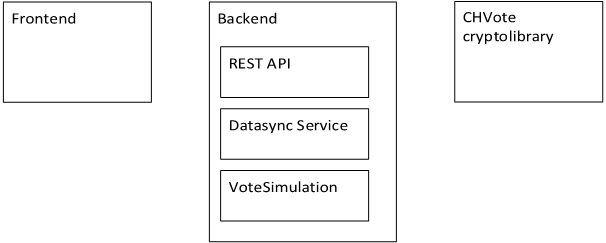
\includegraphics[scale=0.95]{assets/componentdiagram.png}
\caption{System components}
\end{center}
\end{figure}
The \textbf{CHVote crypto-library} is the result of our "`Project 2"' course project which we have finished before our bachelor thesis. This library contains all the algorithms that we have implemented according to the specification. 

The back-end consists of several services that are responsible for simulating a CHVote election, providing an API to manipulate this state and a data sync service to synchronize the data between the clients and the back-end. All the services of the backend run on a single server.

The front-end basically is the web-app where all the functionality of our back-end is consumed and the resulting election state is visualized.
\section{Technology \& Language Decisions}
When we implemented the CHVote crypto-library, we have evaluated and decided to use Python. Since Java has already been used by the team in Geneva, we wanted to use a different language as it was desirable to prove that the CHVote specification can be implemented in any language. Python seemed like a rather suitable language due to the following reasons:
\begin{itemize}	
	\item mature language with lots of libraries
	\item python's syntax enables programs to be written in a compact and readable style
	\item as the protocol wasn't completely specified at that point and has still been undergoing some changes, we wanted to use a language in which we can adapt changes quickly and easily
	\item native support for large integers (\textit{BigInts}) and bindings for the GMP\footnote{GMP is a free library for arbitrary precision arithmetic, operating on signed integers, rational numbers, and floating-point numbers, see \url{https://gmplib.org/}.} library
	\item supports a lot of platforms
	\item many popular web development frameworks are available
\end{itemize}

Throughout the project not all of the reason above turned out to be true or ideal. The drawbacks that we have experienced during the implementation of this project will be discussed at the end of this document.

Since we used the crypto-library in our back-end, Python was also the obvious language for the back-end. Python offers a wide variety of frameworks for building web-services. Since we planed on building a single-page-application for the client, we chose the lightweight micro-framework flask for building a restful web-service. 

For our \textbf{front-end} (web application) we evaluated several single-page application (SPA) frameworks. VueJS is a new, modern and lightweight SPA framework that in contrast to Angular has a much flatter learning curve but still offered all the functionality that we needed. The VueJS addon Vuex enabled us to establish a data-store pattern in our front-end, which makes it possible to have a copy of the back-end data-store in our web application which is synchronized in real-time through web-sockets.

\textbf{Socket.io} simplifies the usage of web-sockets and offers fallback technologies such as long-polling in case web-socket is not supported by either the browser or the web-server. Both Flask as well as VueJS have plug-ins that support and integrate socket.io.

For persisting the state of an election, we decided to use mongoDB. The reason behind this choice will be described in more details later on.

\section{Architecture}
The core of our application is the VoteSimulation component in our backend which implements the e-voting protocol by utilizing all algorithms of the CHVote crypto-library according to the CHVote specification. The VoteSimulation component internally holds the state of a whole CHVote election and exposes functions to manipulate this state at a granularity required by our web application to implement all use cases. For example: The VotingSimulation contains a list of ballots and exposes functions to cast a new ballot, which will generate a new ballot according to the protocol, by calling the CHVote crypto-library, and adds the ballot to the list.

On top of the VoteSimulation we have implemented a REST service that acts a facade to the VoteSimulation component and makes its functionality available as an API for our web-clients. The REST service also has to initialize the VoteSimulation by loading and persisting it's state from and to the database between each API call.

One of the requirements is that all clients must be informed in real-time about mutations of the election state made by other clients. To achieve this, we have implemented a data sync service which allows to push the state or parts of the state of the VoteSimulation to the web-clients by using the websocket protocol. This service is triggered by the REST service after every API call to push the delta between the old and the new state to the clients.

To establish a proper separation of concerns, the state of the VoteSimulation is always sent to the client via the data sync service. The REST service only returns success or error codes or information that is required in response to some particular API call, and never state objects. On the other hand, the data sync service does never manipulate the state of the VoteSimulation and is solely responsible for sending data to the client.

\begin{figure}[h!]
\begin{center}
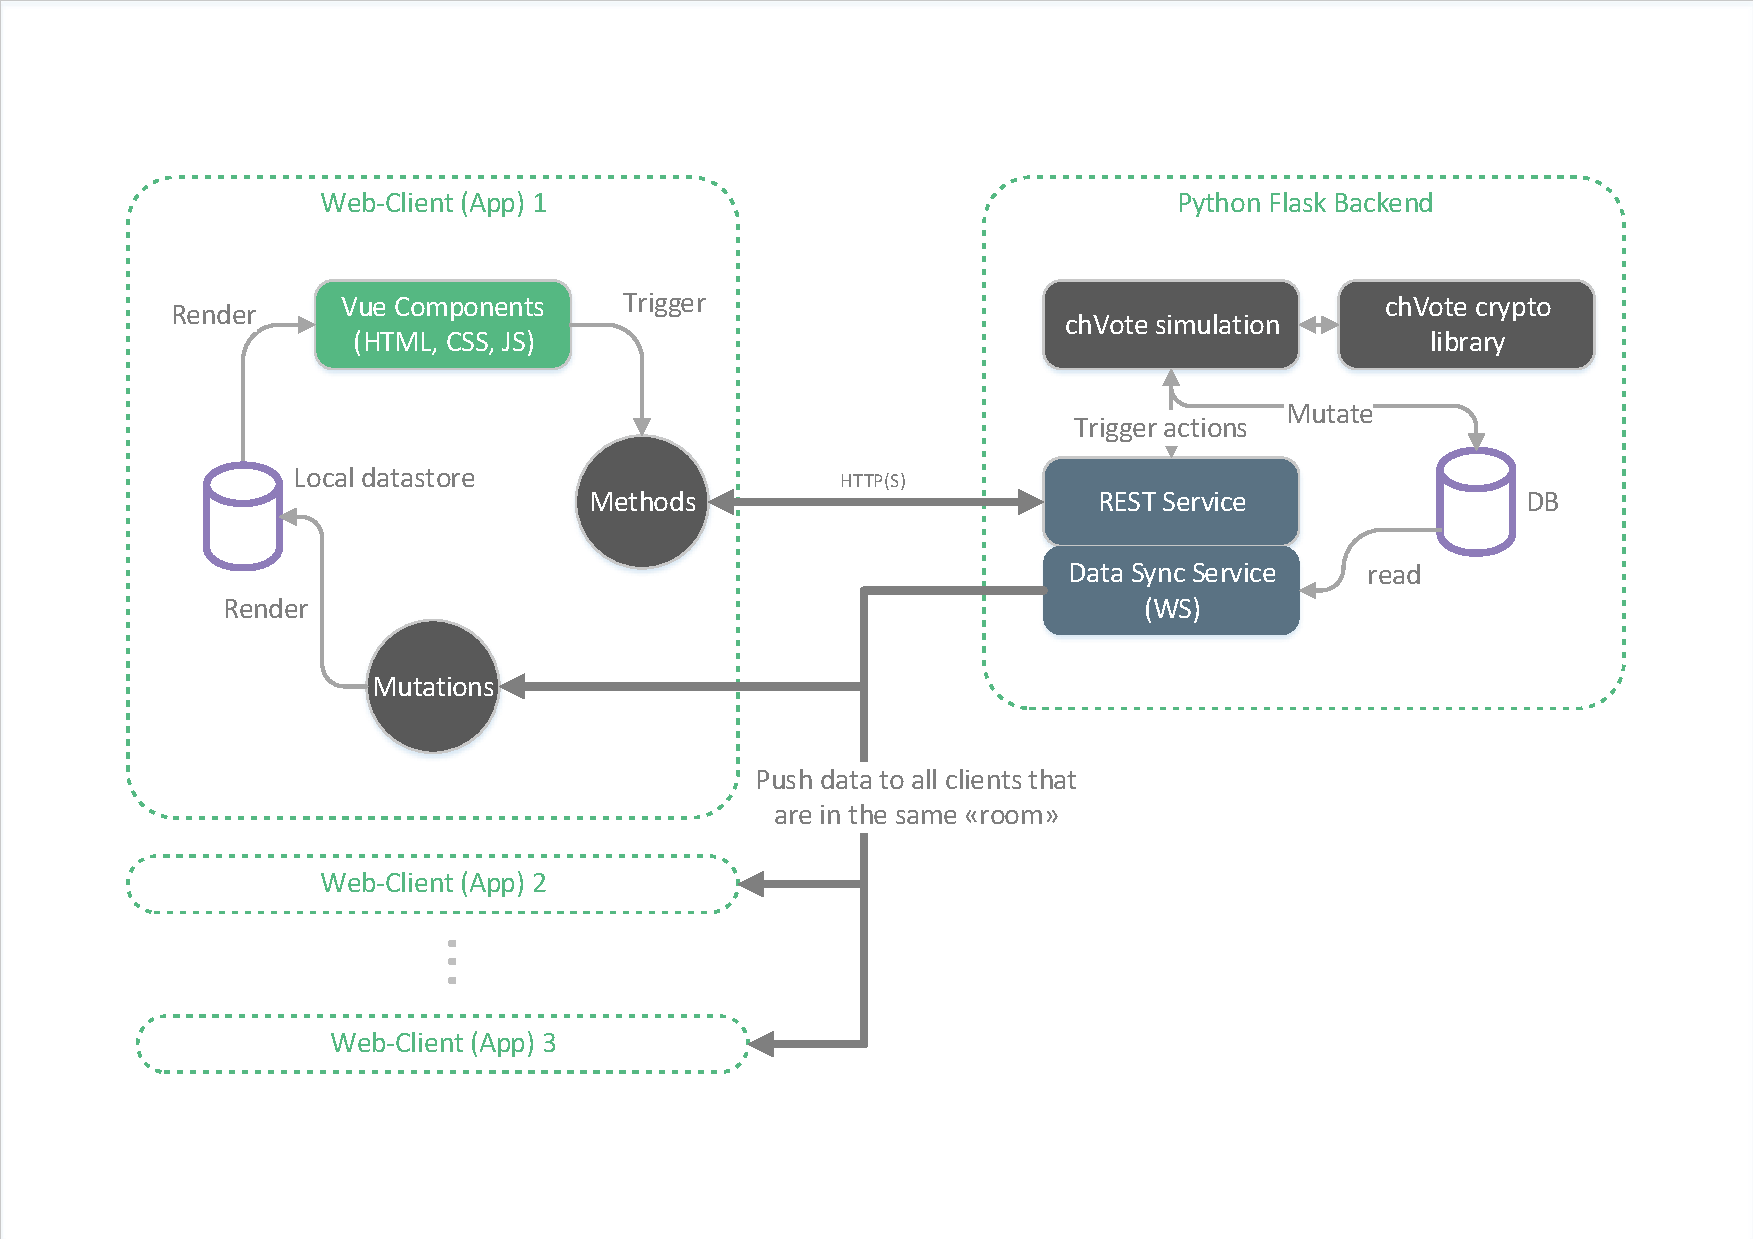
\includegraphics[scale=0.62]{assets/architecture.pdf}
\caption{Architecture}
\end{center}
\end{figure}

From the clients point of view, the web-client contains a copy of the whole VoteSimulation state in a local datastore. This store is initially populated when the web application is initialized with an election. Whenever the state of the VoteSimulation changes, the data sync service is is called to push the new data to the web application. A local mutation handler is called inside the web application which writes the new data into the local datastore.

Since the components that the web-pages of the web application are built of, are directly bound to the local data-store, all mutations automatically reflected to the user. From those pages, the REST API can be called to trigger some CHVote specific action on the back end. The resulting state change is again being pushed to all clients while the responsible client that performed the HTTPS request will additionally receive a success code, or an error message in case of an error.

\section{Back-end}
In this section we describe the internals of the back-end services. 
\subsection{VoteSimulation}
The VoteSimulation represents the state of a whole election and consists of instances of all the actors that participate in a CHVote election. We have divided the state and actors of a CHVote election into the following classes:

\begin{figure}[h!]
\begin{center}
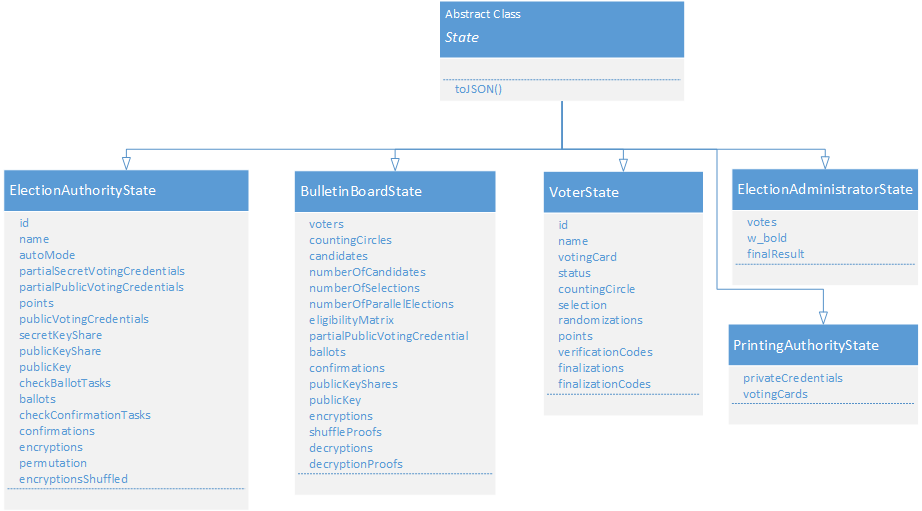
\includegraphics[scale=0.75]{assets/stateClasses.png}
\caption{State classes}
\end{center}
\end{figure}

\begin{itemize}
	\item \textbf{BulletinBoardState}: Holds all data that is publicly available on the bulletin board (the number of candidates, the tallied result)
	\item \textbf{ElectionAuthorityState}: Holds all data that an election authority knows (e.g. the list of ballots, the secret key of an election authority)
	\item \textbf{VoterState}: Since there is no distinction made between a voter and a voting client in our application, the VoterState contains the data of both the voter (e.g. the voting card) and the data typically known to the voting client (e.g. the points returned by the oblivious transfer)
	\item \textbf{PrintingAuthorityState}: Holds the data known to the printing authority (e.g. the list of all voters private credentials and the voting cards)
	\item \textbf{ElectionAdministratorState}: Holds all data known to the election administrator 
\end{itemize}

Since our application must handle multiple elections in parallel, the state cannot be kept in RAM, but needs to be persisted between every single request. For this reason we evaluated different database systems and concepts. We decided not to use a relational database system that requires us to define a database schema as we want our state objects to be the only place where the schema is defined. This makes it easier to apply changes to the protocol in future. 

For our purpose, mongoDB seemed like a good choice. Since we do not need the ability to access and filter our data with arbitrary queries, but only need to be able to save and load a state object of a particular election, we simply store the whole state as a binary string in a mongoDB collection. The only additional attribute that is saved to the database alongside with the serialized state is the electionId which denotes which election a particular state belongs to. 

An election contains multiple VoterStates and ElectionAuthorityStates. Therefore, these two states additionally require an electionAuthorityId and a voterId.

\begin{figure}[h!]
\begin{center}
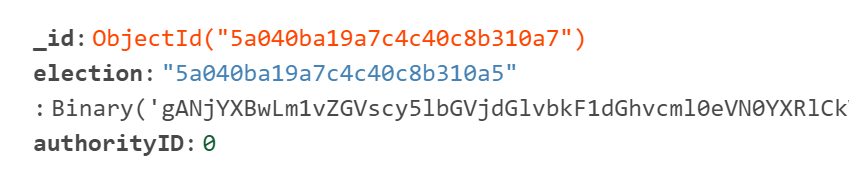
\includegraphics[scale=0.62]{assets/db.png}
\caption{Example: ElectionAuthority document collection}
\end{center}
\end{figure}

The only common functionality between every state object, is the ability to serialize the object to a JSON string. For this reason we had to write a custom transformer which tells the JSON parser how to serialize data-types such as mpz, bytearrays and custom classes. Luckily, python offers a way to easily serialize any custom object. By calling \mintinline{python}/object.__dict__/ we can convert an object into a dictionary, as long as the transformer is able to serialize all properties of the object.

We described how the state classes are used to divide the data of the VoteSimulation into smaller units. Similarly, the functionality of the VoteSimulation class is separated into classes, one for every actor in the protocol.

\begin{figure}[h!]
\begin{center}
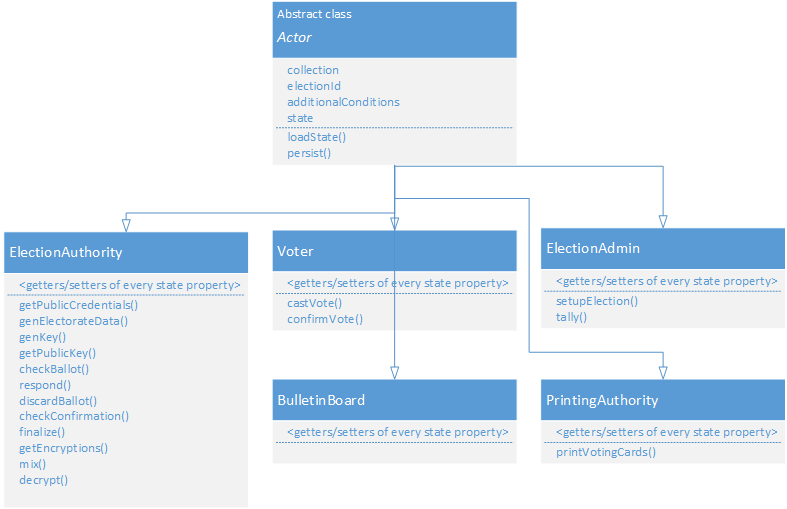
\includegraphics[scale=0.75]{assets/actorClasses.png}
\caption{Actor classes}
\end{center}
\end{figure}

The common functionality, namely, a function for loading the corresponding state from the database and one for persisting the state to the database, are contained in an abstract base class.

The distinction between the actors and their states allows us to easily serialize the state of every actor and provide methods for loading and persisting the state to the database.

\begin{figure}[h!]
\begin{center}
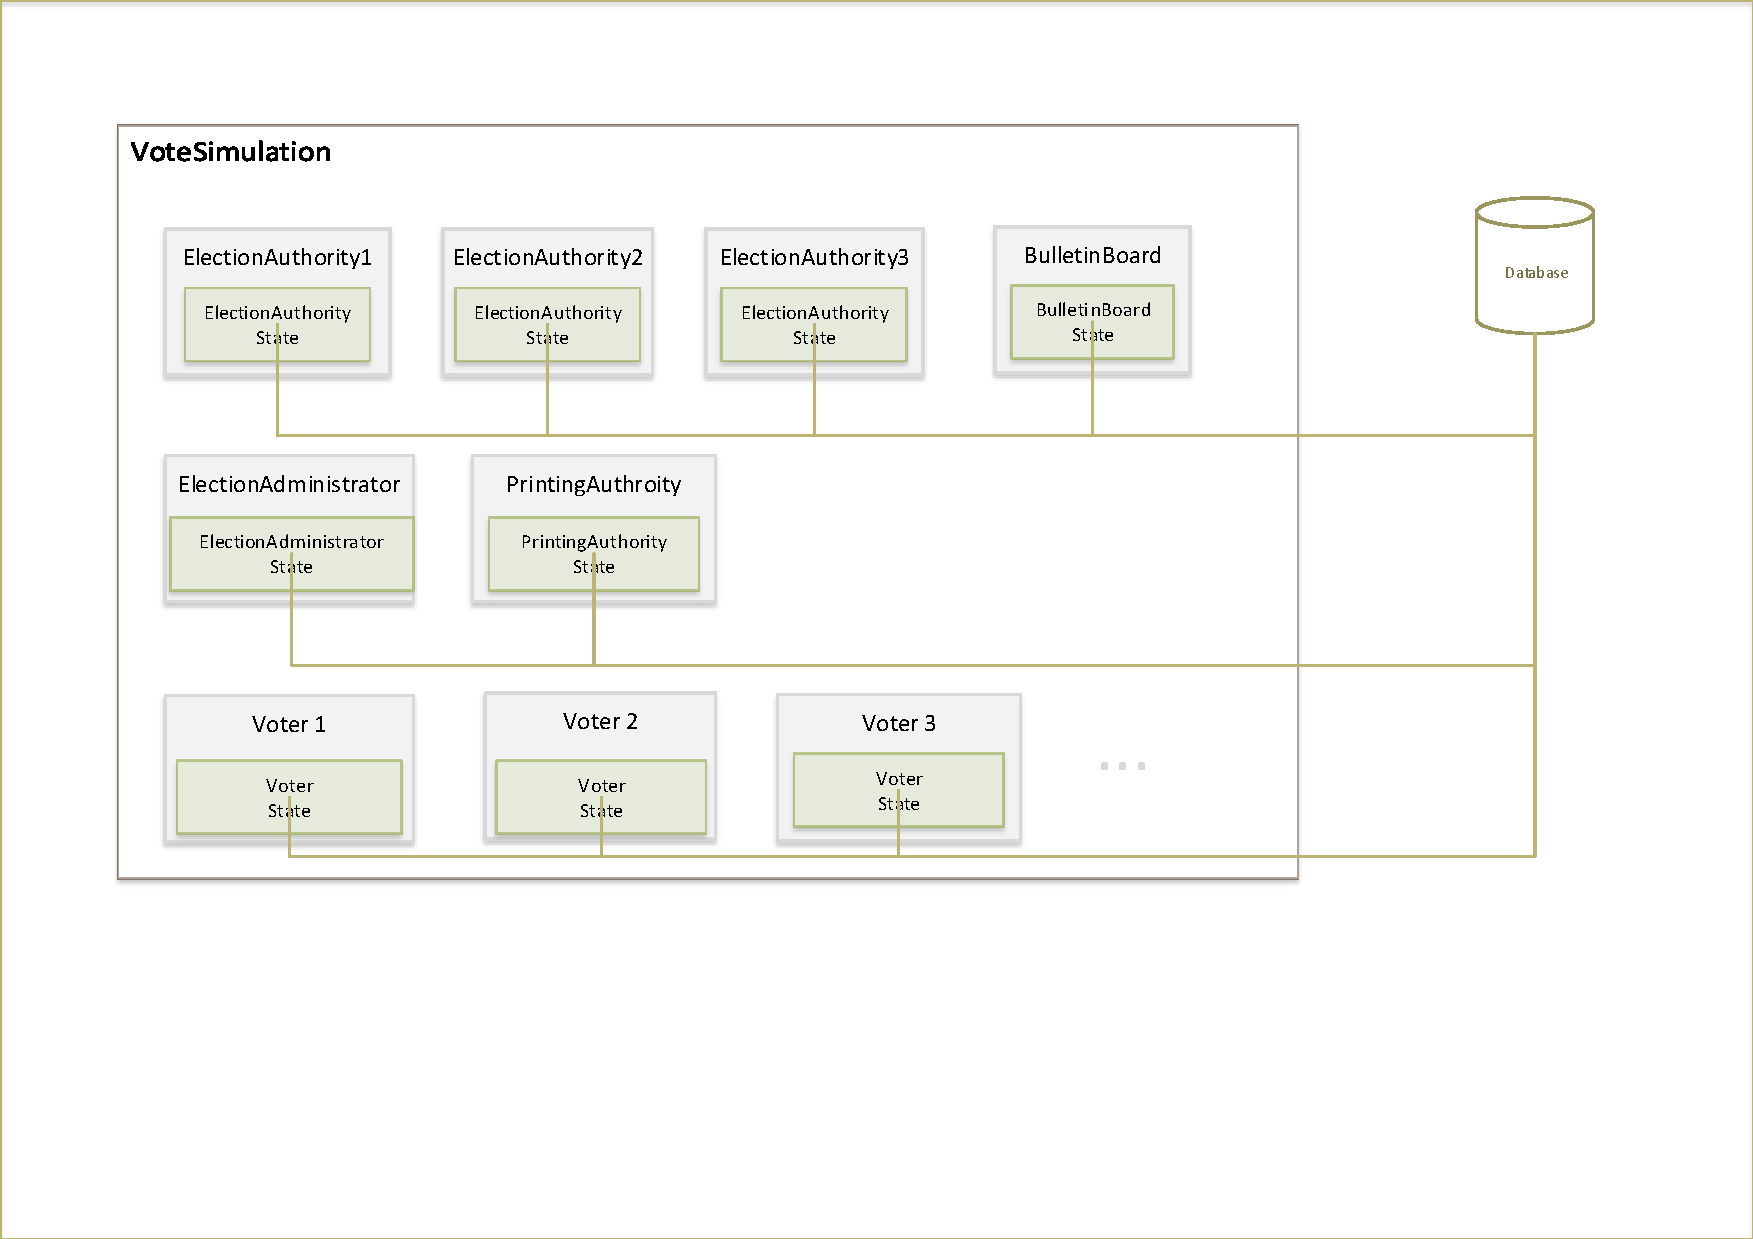
\includegraphics[scale=0.60]{assets/votesim.pdf}
\caption{State classes}
\end{center}
\end{figure}

This approach was also necessary because we have implemented the data synchronization between the clients and the back-end using the JSON Patch approach, for which the delta between the original state and the modified state can be automatically determined and operations generated which will patch the state object on the client such that it equals the new, modified state of the back-end. The original state is simply attached as another property to the actor-object. 

\subsection{Data-Sync Service}
One of the big challenges of our application has been the synchronization of the election state from the back-end to the clients local data store. As mentioned earlier, we wanted to achieve real time data synchronization such that every web client observing a particular election, is informed of any change of this elections state. For this purpose we have used web-sockets.

Additionally, we had to keep an eye on the performance of the data transfers since especially the bulletin board and the election authorities grow big in size when they contain a lot of ballots. We observed that the size of the whole state of an election with 6 candidates and 10 voters, of which each has submitted at least one ballot and a confirmation can easily reach 600 kilobytes already. Admittedly, we haven't noticed any performance issues even with rather large elections, however, transferring the whole state of an election after every single mutation didn't seem like a proper solution.

Nevertheless, when a client connects to the data sync service for the first time, it needs to fetch the JSON representation of every state object of the VoteSimulation. For this purpose we have implemented a "`FullSync"' method which will populate the clients local data store with the full state of an election.

\begin{figure}[h!]
\begin{center}
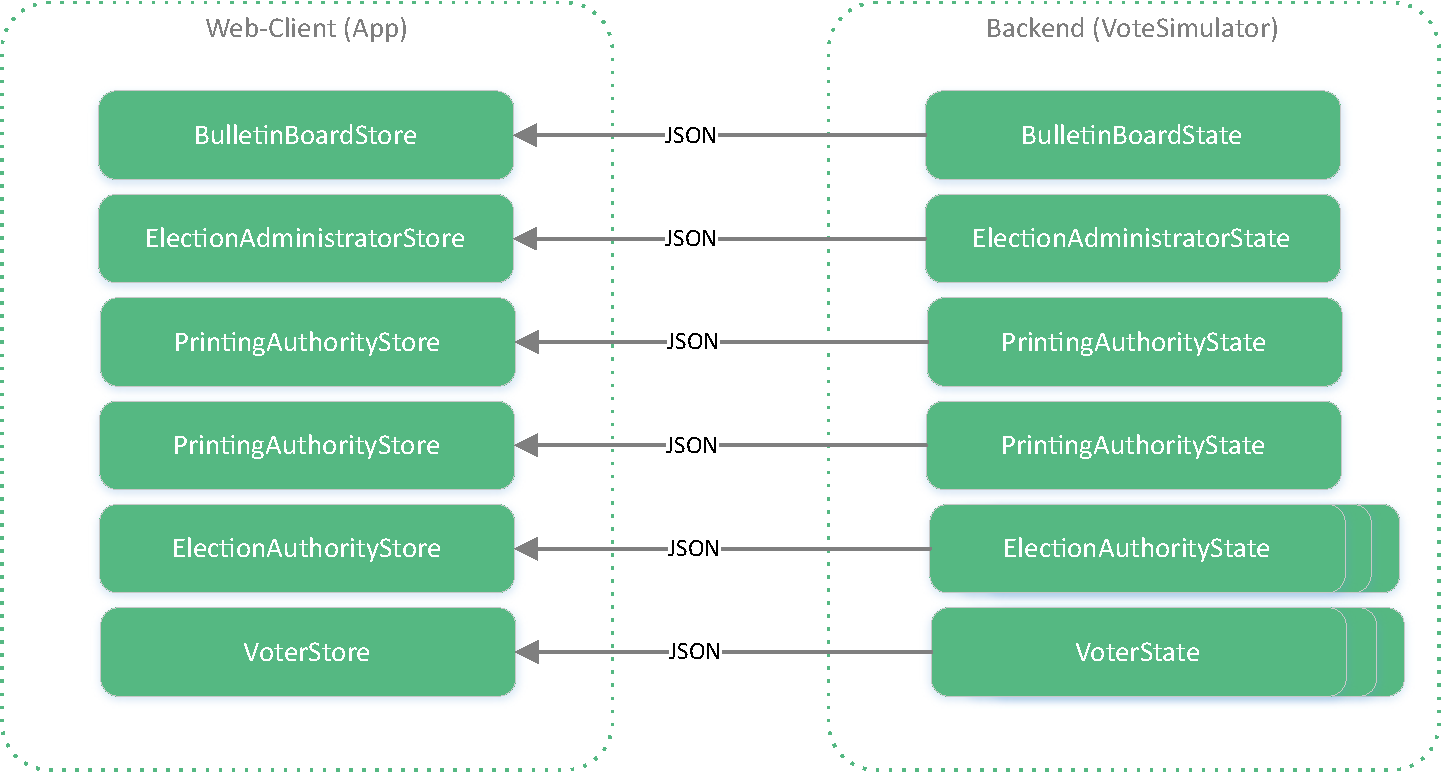
\includegraphics[scale=0.60]{assets/datastores.pdf}
\caption{State classes}
\end{center}
\end{figure}

After a client has pupulated his local data store, future manipulations on the backend are synchronized using the so called JSON Patch operations, which only contain the delta between the previous and the current state.

JSON Patch is a structure for describing how a JSON document can be modified / "`patched"'. The procedure is standardized and described in the RFC 6902 of the Internet Engineering Task Force (IETF). There exist JSON Patch implementations for many languages, including Python and JavaScript. We used JSON Patch to realize our incremental data synchronization as follows:

When the VoteSimulation loads the state of its actor objects, it sets the \mintinline{python}/originalState/ property of the actor to a deep copy of the loaded state object. Mutations are always done only to the \mintinline{python}/state/ property. Before calling the \mintinline{python}/persist()/ method on an actor object, we use the Python JSON Patch library to create a set of JSON Patch operations that describes how to patch the \mintinline{python}/originalState/ such that it becomes identical to the manipulated \mintinline{python}/state/ object, by calling 
\mintinline{python}/make_patch(json.loads(self.originalState.toJSON()), json.loads(self.state.toJSON()))/

The result is a JSON array of operations that contains:
\begin{itemize}
	\item The path of the manipulation
	\item The type of operation (replace, add, remove, ...)
	\item The new value (if required)
\end{itemize}

For example, after casting a ballot, we might receive the following JSON patch:

\begin{figure}[h!]
\begin{center}
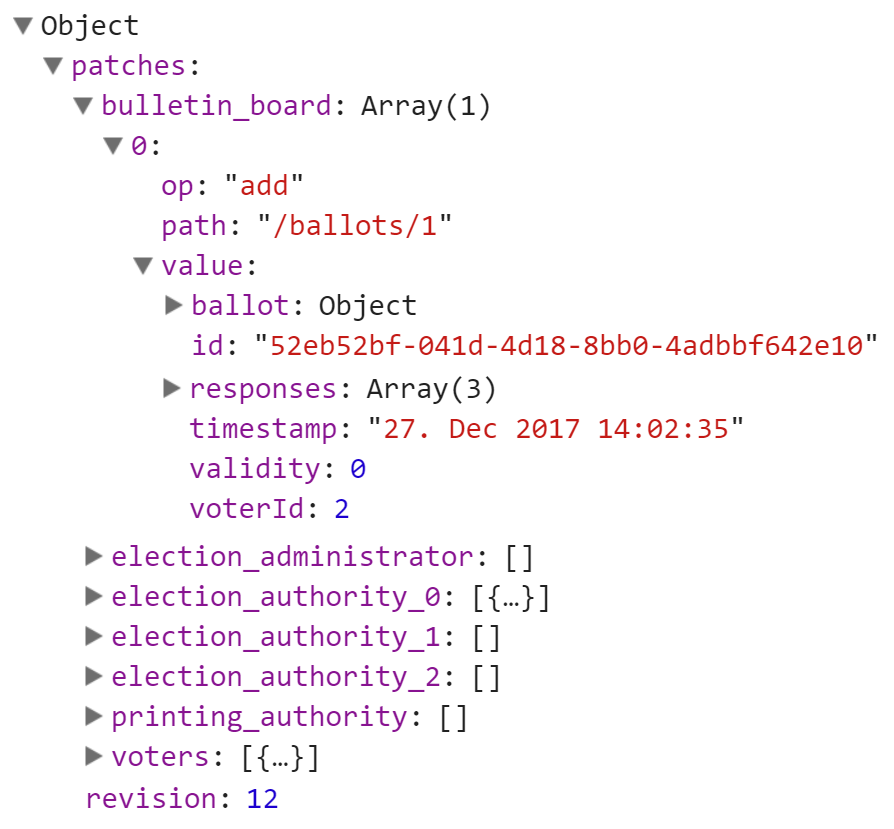
\includegraphics[scale=1]{assets/jsonpatchexample.png}
\caption{JSON Patch example}
\end{center}
\end{figure}

These JSON patches are pushed to all the clients that need to receive the mutations and are applied to the local datastore which contains the original state. After applying the JSON patch, the data store of all clients contains the same state of an election as the backend.

\begin{figure}[h!]
\begin{center}
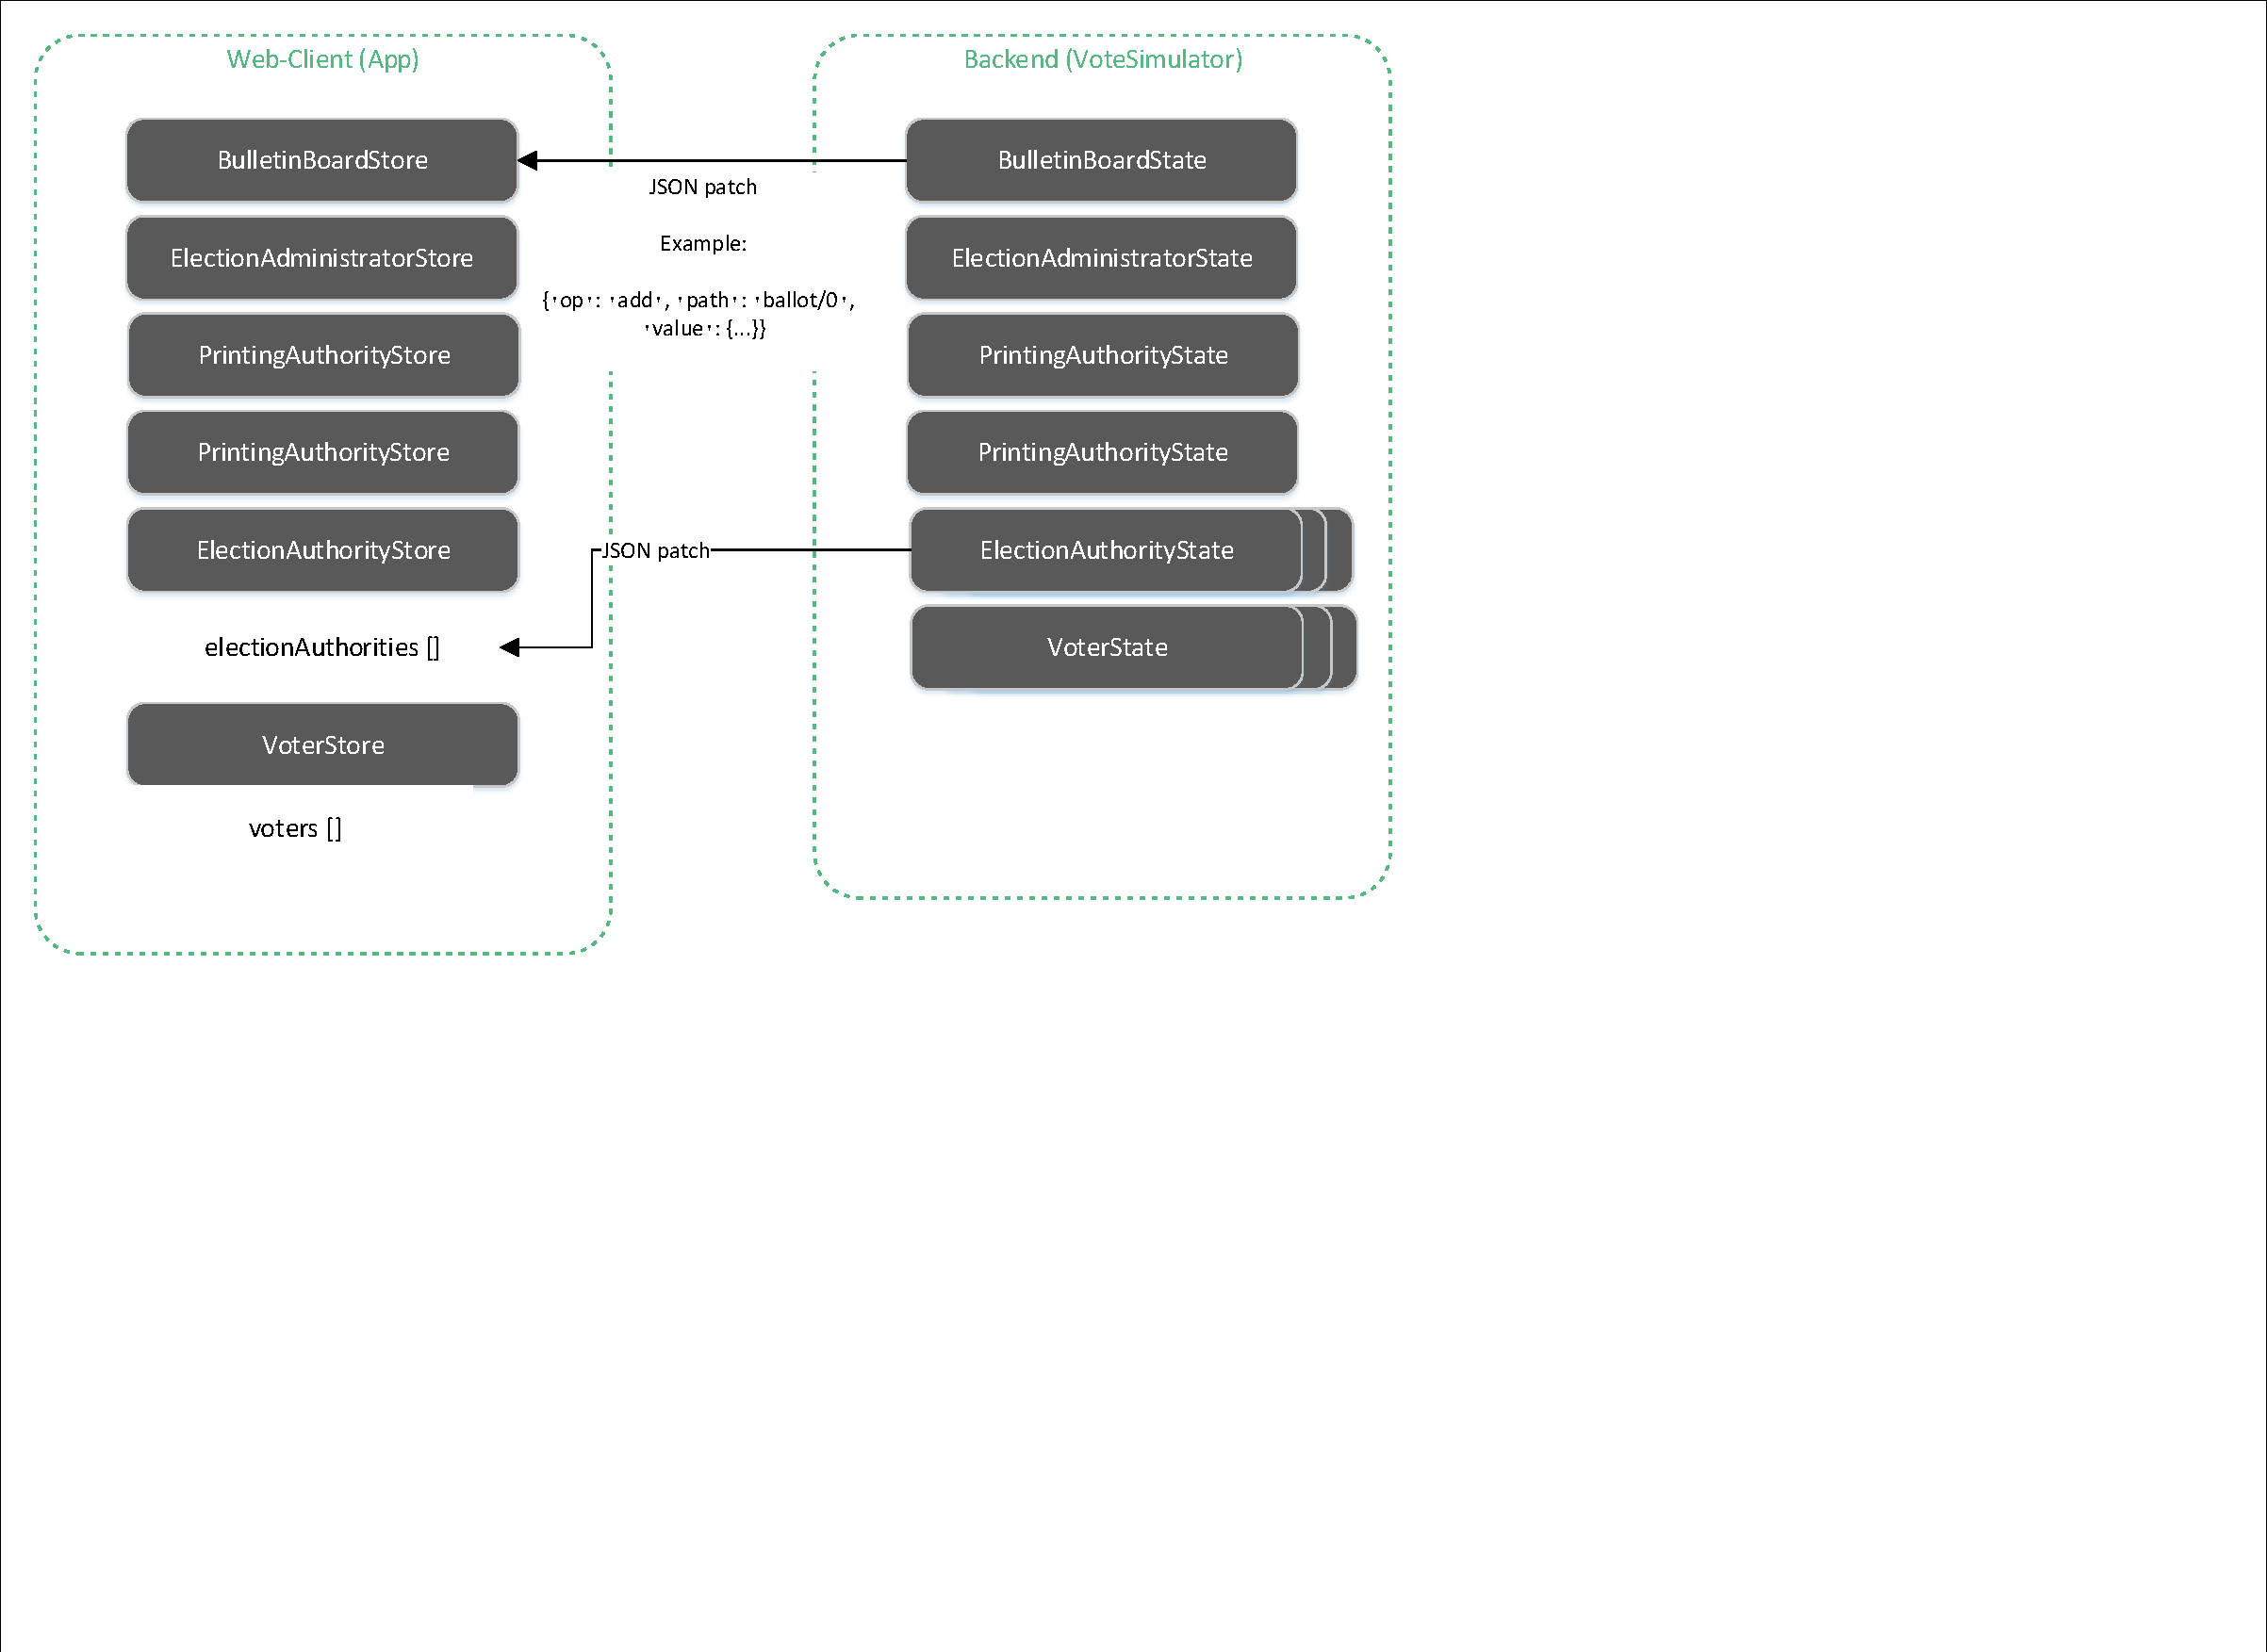
\includegraphics[scale=0.60]{assets/datastores_jsonpatch.pdf}
\caption{Data-Sync with JSON Patches}
\end{center}
\end{figure}

We decided not to use JSON patches when populating the data store for the first time, since generating JSON patches to patch an empty object to the full state of an election could result in thousands of operations that would almost certainly perform worse than sending the whole object over a fast websocket connection.

\subsection{REST API}
The third component of the backend is the REST API. Its responsibility is to serve as an API and to provide all the functionality of the VotingSimulation to the webclients. Every function, such as the \mintinline{python}/castVote()/ has a corresponding endpoint in the REST API service. Since almost every API endpoint looks almost the same, we take a look at one of them:

\begin{minted}[linenos,tabsize=2,breaklines]{python}
@main.route('/castVote', methods=['POST'])
@cross_origin(origin='*')
def castVote():
    data = request.json
    electionId = data["election"]
    selection = data["selection"]
    voterId = data["voterId"]
    votingCode = data["votingCode"]

    if len(selection) == 0:
        return make_error(400, "Empty selection")

    try:        
        sim = VoteSimulator(electionId) # prepare voteSimulator
        
        sim.castVote(voterId, selection, votingCode) # perform action
        
        patches = sim.persist()	# persist modified state and retrieve JSON patches
        
				syncPatches(electionId, SyncType.ROOM, patches)	# send the JSON patches to all clients

    except Exception as ex:
        return make_error(500, str(ex))

    return json.dumps({'result': 'success'})
\end{minted}

The API can be reached by sending a HTTP(S) POST request to our webserver hosting the backend. The URL defines what function will be executed. For example: A POST request to https://<server>:5000/castVote/ would call the above function. The required parameters are added in the POST body.

As a first step, parameters are extracted from the POST request and validated if necessary. As the next step , a VoteSimulator object is instantiated by passing the electionId to the constructor. The VoteSimulator will internally load the states of the corresponding election from the database and instantiate the actor objects such as the election authorities.

Now the VoteSimulator can execute the function which the user intended to call, for example "`CastVote"'. By calling the function \mintinline{python}/persist()/, the new state is written to the database and the JSON Patches of all mutations are determined, returned and can be sent to all clients by calling the Data-Sync service.

The following sequence diagram shows how the vote casting use case is implemented within the backend and how all the components work together.
\begin{figure}[h!]
\begin{center}
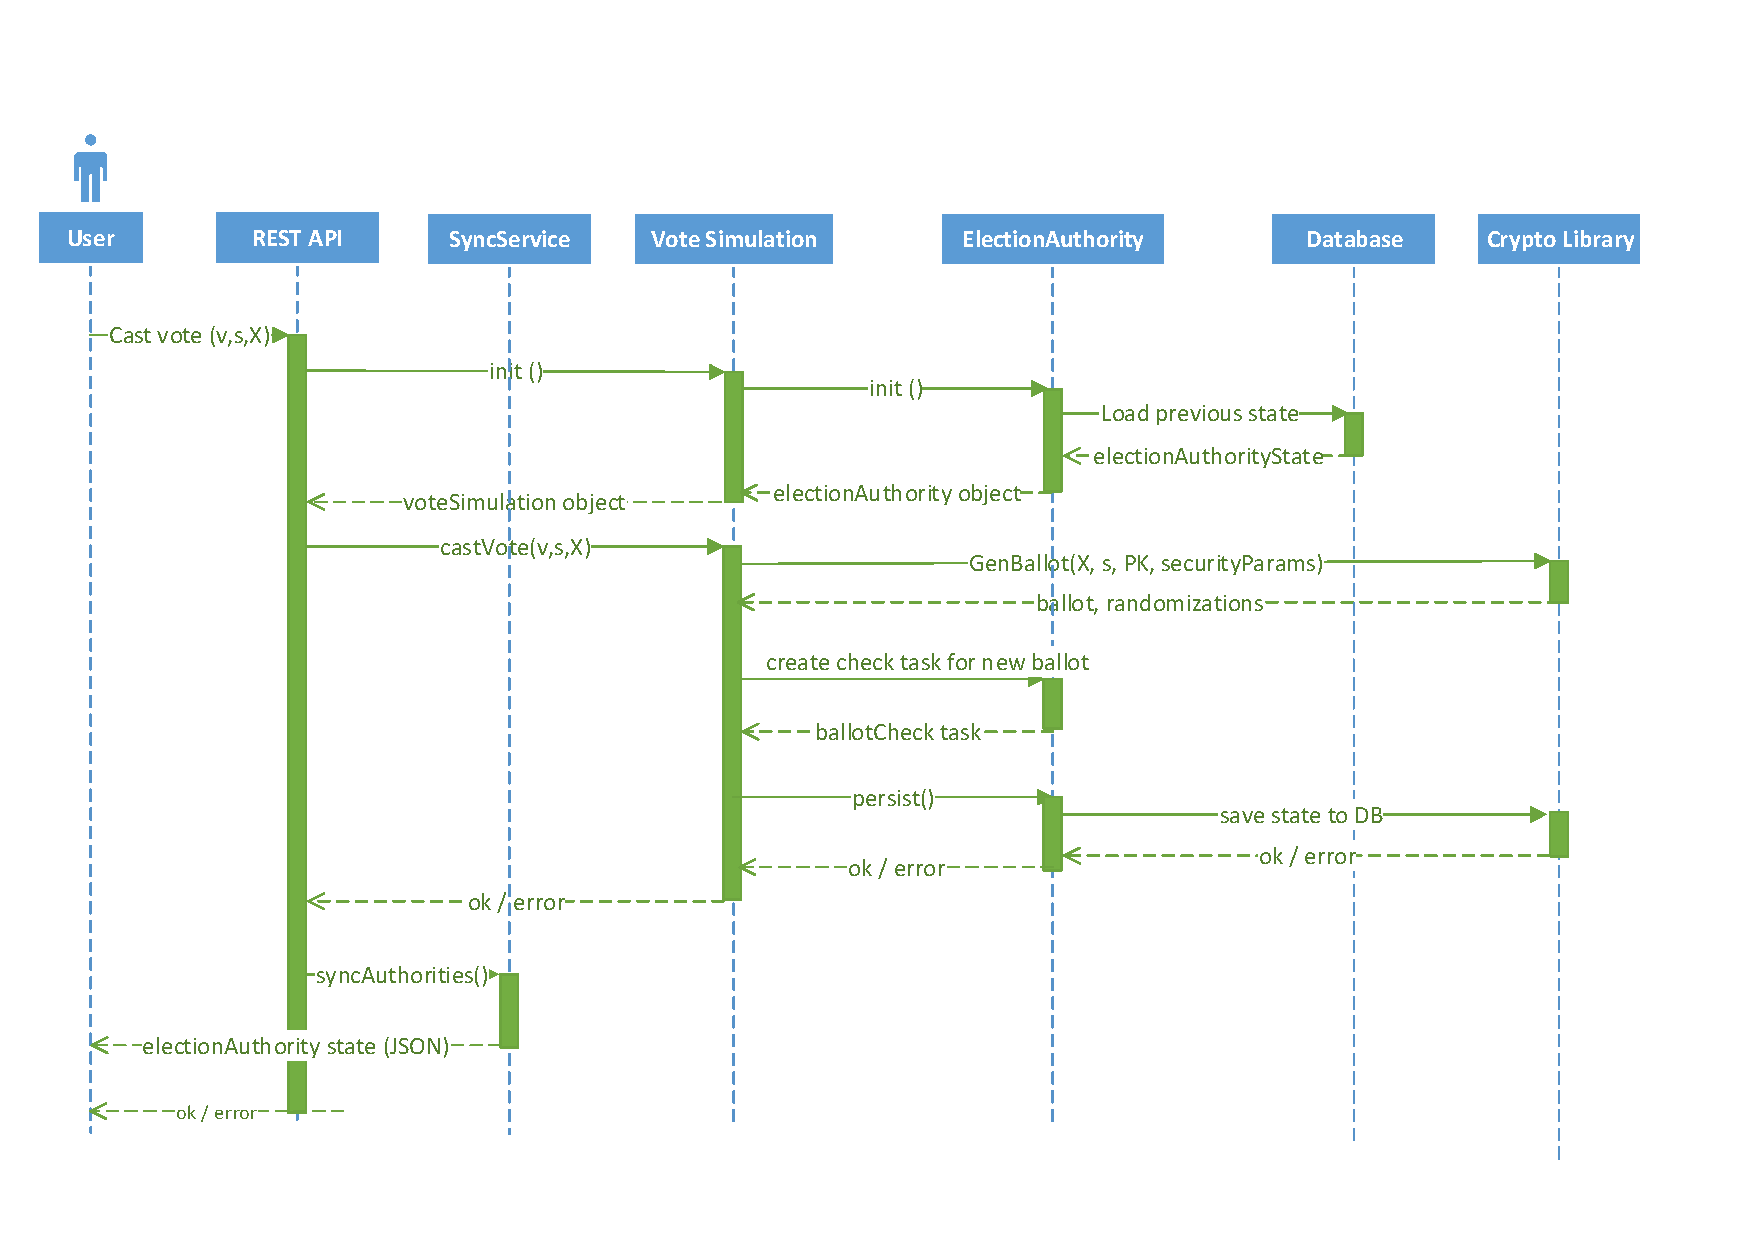
\includegraphics[scale=0.65]{assets/votecastingDiagram.pdf}\\
\caption{Vote casting sequence diagram}
\end{center}
\end{figure}

\section{Crypto-library}

\subsection{File structure}
We decided to put every algorithm of the specification in its own file together with related unit tests. The files are structured according to the actors of the protocol, for example:

\begin{itemize}
	\item \textbf{Common}: contains common cryptopgraphic algorithms and the security parameters used by multiple algorithms
	\item \textbf{ElectionAuthority}: contains all the algorithms used by the election authority
	\item \textbf{PrintingAuthority}: contains all the algorithms used by the printing authority
	\item \textbf{VotingClient}: contains all the algorithms used by the voting client
	\item \textbf{ElectionAdministration}: contains all the algorithms used by the election administrator
	\item \textbf{Utils}: contains helper classes and miscellaneous utility functions
\end{itemize}

\subsection{Public parameters}
There exist two types of public parameters:

The \textbf{security relevant parameters}, e.g:

\begin{itemize}
	\item The order of the prime groups: $p$, $\prime{p}$, $\hat{p}$
	\item The length of the voting, confirmation, return and finalization codes
	\item The number of authorities: $s$
\end{itemize}

and \textbf{public election parameters}, e.g.:

\begin{itemize}
	\item The size of the electorate: $N_E$
	\item The number of candidates: $n$
	\item The list of candidate descriptions: $c$
\end{itemize}

The security parameters are typically used within the algorithms and remain unchanged for a longer time period, whereas the public election parameters are only used by the protocol implementations and change with every election.

The object \texttt{SecurityParams} holds all security relevant parameters and is injected as an additional function argument to all algorithms. Several different \texttt{SecurityParams} objects are created initially, which contain all the parameters according to the recommendations in the CHVote specification document ("level 0" for testing purposes and "level 1" through "level 3" for actual use of the protocol). This approach allows us to use different levels of security during development of the algorithms and protocols. For simple unit testing we used "level 0" in order to inject the security parameters recommended for testing puposes. For actual test runs of the project the security parameters from "level 2" were used.

The public election parameters on the other hand are directly passed to the algorithms by the calling party. If an algorithm needs to know certain election parameters (like the size of the electorate $N_E$), these values are typically derived from vectors that they have access to, so they do not require specific knowledge of these parameters.

\subsection{Coding style}
The following source code sample shows a typical implemation of an algorithm (in this exmaple, algorithm 7.18 according to the CHVote specification).

\begin{minted}[linenos,tabsize=2,breaklines]{python}
import unittest
import os, sys
from gmpy2 import mpz
import gmpy2

sys.path.append(os.path.dirname(os.path.dirname(os.path.abspath(__file__))))

from Utils.Utils                    import AssertMpz, AssertList, AssertClass, AssertString
from Crypto.SecurityParams          import SecurityParams, secparams_l0
from Utils.ToInteger                import ToInteger
from VotingClient.GetSelectedPrimes import GetSelectedPrimes
from VotingClient.GenQuery          import GenQuery
from VotingClient.GenBallotProof    import GenBallotProof
from UnitTestParams                 import unittestparams
from Types                          import Ballot
from Utils.StringToInteger          import StringToInteger

def GenBallot(X_bold, s, pk, secparams):
    """
    Algorithm 7.18: Generates a ballot based on the selection s and the voting code X. The
    ballot includes an OT query a and a proof pi. The algorithm also returns the random
    values used to generate the OT query. These random values are required in Alg. 7.27
    to derive the transferred messages from the OT response, which itself is generated by Alg. 7.25.

    Args:
        X_bold (str):                       Voting Code X ∈ A_X^l_X
        s (list of int):                    Selection s = (s_1, ... , s_k), 1 <= s_1 < ... < s_k
        pk (mpz):                           ElGamal key pk ∈ G_p \ {1}
        secparams (SecurityParams):         Collection of public security parameters

    Returns:
        tuple:                              alpha = (r, Ballot) = (r, (x_hat, a, b, pi))
    """

    AssertMpz(pk)
    AssertList(s)
    AssertClass(secparams, SecurityParams)

    x = mpz(StringToInteger(X_bold, secparams.A_X))
    x_hat = gmpy2.powmod(secparams.g_hat, x, secparams.p_hat)

    q_bold = GetSelectedPrimes(s, secparams)                    # q = (q_1, ... , q_k)
    m = mpz(1)

    for i in range(len(q_bold)):
        m = m * q_bold[i]

    if m >= secparams.p:
        return None

    (a_bold, r_bold) = GenQuery(q_bold, pk, secparams)
    a = mpz(1)
    r = mpz(0)

    for i in range(len(a_bold)):
        a = (a * a_bold[i]) % secparams.p
        r = (r + r_bold[i]) % secparams.q

    b = gmpy2.powmod(secparams.g,r, secparams.p)
    pi = GenBallotProof(x,m,r,x_hat,a,b,pk, secparams)
    alpha = Ballot(x_hat,a_bold,b,pi)

    return (alpha, r_bold)

class GenBallotTest(unittest.TestCase):
    def testGenBallot(self):
        selection = [1,4]       # select candidates with indices 1,4
        (ballot, r) = GenBallot(unittestparams.X, selection, unittestparams.pk, secparams_l0)
        print(ballot)
        print(r)

if __name__ == '__main__':
    unittest.main()
\end{minted}

All algorithms contain a short description, which was taken as-is from the specification document, as well as a comment (Google-style documentation string), which can be used to automatically generate code documentation. The algorithm itself is implemented as close to the specification as possible, using the same variable names and (as far as the language supports it) similar control structures:

\begin{itemize}
	\item The suffix \texttt{\_bold} for emphasized (bold) variables, e.g. \texttt{p\_bold} for \textbf{p}
	\item The suffix \texttt{\_hat} for variables with a hat, e.g. \texttt{a\_hat} for $\hat{a}$
	\item The suffix \texttt{\_prime} for variables with a prime, e.g. \texttt{a\_prime} for $a'$
	\item etc.
\end{itemize}

Each file also contains unit test relevant to the specific algorithm (if unit testing was considered useful for the particular algorithm).

The following example shows the similarities between the algorithm pseudo code and the actual implmentation in Python:

\begin{multicols}{2}
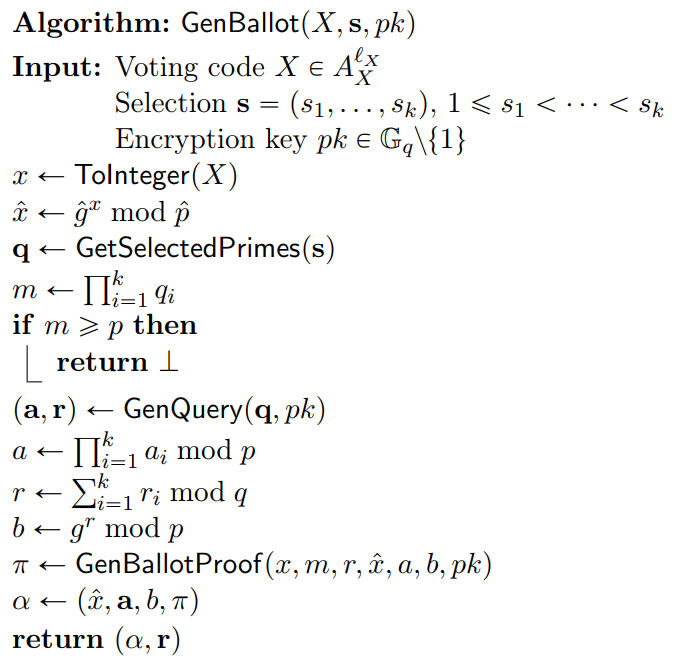
\includegraphics[width=0.46\textwidth]{assets/genballot.png}
\columnbreak
\begin{minted}[fontsize=\scriptsize]{python}
x = mpz(StringToInteger(X_bold, secparams.A_X))
x_hat = gmpy2.powmod(secparams.g_hat, x, secparams.p_hat)
q_bold = GetSelectedPrimes(s, secparams)

m = mpz(1)
for i in range(len(q_bold)):
    m = m * q_bold[i]

if m >= secparams.p:
    return None

(a_bold, r_bold) = GenQuery(q_bold, pk, secparams)
a = mpz(1)
r = mpz(0)

for i in range(len(a_bold)):
    a = (a * a_bold[i]) % secparams.p
    r = (r + r_bold[i]) % secparams.q

b = gmpy2.powmod(secparams.g,r, secparams.p)
pi = GenBallotProof(x,m,r,x_hat,a,b,pk, secparams)
alpha = Ballot(x_hat,a_bold,b,pi)

return (alpha, r_bold)
\end{minted}
\end{multicols}

\subsection{Return types}
In most cases, when an algorithm returns more than a scalar datatype, tuples are used. Tuples allow to return multiple values from a function:

\begin{minted}[linenos,tabsize=2,breaklines]{python}
def foo():
   return (1, 2)

def main():
   a, b = foo()
\end{minted}

This way a lot of the source code looked very similar to the pseudo code in the CHVote specification. For more complex data types or return values that are used more often, named tuples were used. The data type "namedtuple" is like a lightweight class and allows access to named properties.

\begin{minted}[linenos,tabsize=2,breaklines]{python}
Ballot = namedtuple("Ballot", "x_hat, a_bold, b, pi")

def main():
   Ballot b = getBallot()
   x_hat = b.x_hat
\end{minted}

By following this approach we can avoid having lots of container classes only used to pass data structures between the algorithms.

\section{Frontend}
Our frontend is a singlepage application built with Javascript, VueJS, HTML5 and CSS3. We tried to follow the design patterns and best practices proposed by the VueJS framework wherever possible.

Every site of our applications consists of at least one VueJS component which is activated when the user visits the corresponding route in the URL.
\subsection{Datastore}
The web application's datastore is divided into multiple modules, one datastore module for each corresponding state of the backend.

TODO: Grafik die zeigt, wie VueX Datastores mit Backend States zusammenhängen
 
\subsection{Websocket room concept}
TODO: Konzept mit den Rooms / Election IDs beschreiben

\subsection{Development Environment}
TODO: Webpack, ESlint etc. beschreiben